\usetikzlibrary{arrows.meta}
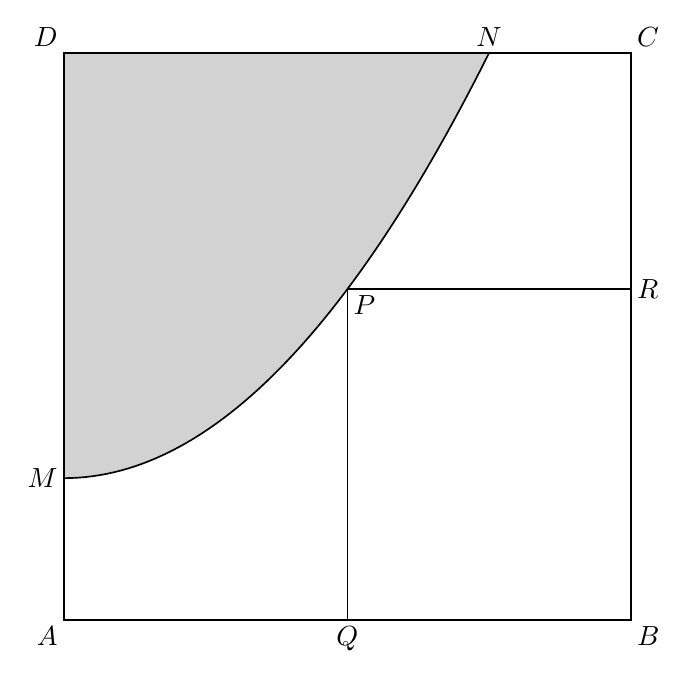
\begin{tikzpicture}[x=18mm,y=18mm,line width=.6pt,font=\normalsize,>=Stealth]
\def\qx{2}
\pgfmathsetmacro{\py}{\qx*\qx/3+1}
\fill[gray!35] (0,4) -- (3,4) -- plot[domain=3:0,samples=60] (\x,{\x*\x/3+1}) -- cycle;
\draw (0,0) rectangle (4,4);
\draw[domain=0:3,samples=60] plot (\x,{\x*\x/3+1});
\draw (4,0) -- (\qx,0) -- (\qx,\py) -- (4,\py) -- cycle;
\node[inner sep=0pt,anchor=north east,xshift=-2pt,yshift=-2pt] at (0,0) {$A$};
\node[inner sep=0pt,anchor=north west,xshift=2pt,yshift=-2pt] at (4,0) {$B$};
\node[inner sep=0pt,anchor=south west,xshift=2pt,yshift=2pt] at (4,4) {$C$};
\node[inner sep=0pt,anchor=south east,xshift=-2pt,yshift=2pt] at (0,4) {$D$};
\node[inner sep=0pt,anchor=east,xshift=-2pt] at (0,1) {$M$};
\node[inner sep=0pt,anchor=south,yshift=2pt] at (3,4) {$N$};
\node[inner sep=0pt,anchor=north west,xshift=2pt,yshift=-2pt] at (\qx,\py) {$P$};
\node[inner sep=0pt,anchor=north,yshift=-2pt] at (\qx,0) {$Q$};
\node[inner sep=0pt,anchor=west,xshift=2pt] at (4,\py) {$R$};
\end{tikzpicture}
